\documentclass[12pt]{article}
\usepackage[T1]{fontenc}
\usepackage{titling}
\usepackage{pdfpages}
\usepackage{setspace}
\usepackage{graphicx}
\usepackage{amsmath}
\usepackage{circuitikz}
\usepackage{listings}
\lstset{ 
	language=Matlab,                		% choose the language of the code
%	basicstyle=10pt,       				% the size of the fonts that are used for the code
	numbers=left,                  			% where to put the line-numbers
	numberstyle=\footnotesize,      		% the size of the fonts that are used for the line-numbers
	stepnumber=1,                   			% the step between two line-numbers. If it's 1 each line will be numbered
	numbersep=5pt,                  		% how far the line-numbers are from the code
%	backgroundcolor=\color{white},  	% choose the background color. You must add \usepackage{color}
	showspaces=false,               		% show spaces adding particular underscores
	showstringspaces=false,         		% underline spaces within strings
	showtabs=false,                 			% show tabs within strings adding particular underscores
%	frame=single,	                			% adds a frame around the code
%	tabsize=2,                				% sets default tabsize to 2 spaces
%	captionpos=b,                   			% sets the caption-position to bottom
	breaklines=true,                			% sets automatic line breaking
	breakatwhitespace=false,        		% sets if automatic breaks should only happen at whitespace
	escapeinside={\%*}{*)}          		% if you want to add a comment within your code
}
\graphicspath{ {./images/} }


\begin{document}

\setlength{\droptitle}{-10em}
\title{Problem Set \#15}
\author{Olorunjuwon Ajayi, Junkyu Kwon}
\date{February 11, 2020}
\maketitle

\section{Problem Description}
An RLC circuit contains a resistor, inductor, and capacitor, connected in series or parallel. The circuit is a harmonic oscillator of current, and the current oscillation maximized when the frequency gets closer to the resonance frequency. 
The object of the problem is to build and measure the performance of a simple RLC oscillator. We measure the oscillations as a function of time and compare the experimental results to what is theoretical expected.

\section{Material}
\begin{enumerate}
  \item ELVIS breadboard
  \item ELVIS oscilloscope
  \item ELVIS function generator
  \item Jumper cables
  \item 1000 K$\Omega$ resistor
  \item 10 nF capacitor
  \item 10 mH inductor
\end{enumerate}

\section{Procedure}
\begin{enumerate}
  \item Set up linear RLC circuit and software
  \item Obtain resonance frequency using $1/2\pi(LC)$ 
  \item Measure time \textit{vs} current graph for resistor
\end{enumerate}

% Figure 2
\begin{figure}[htp]
    \begin{center}
        \begin{circuitikz} 
            \draw
            (0,0) to[sV=$V$] ++ (0,5)
            (0,5) to[R=1000 K$\Omega$] (3,5)
            (3,5) to[L=10 mH] (6,5)
            (6,5) to[C=10 nF] (9,5)
            (9,5) to[short] (9,0)
            (0,0) to[short] (9,0)
            (4,0) node[ground] {};
        \end{circuitikz}
    \end{center}
    \caption{Diagram of the RLC circuit.}
    \label{fig:galaxy}
\end{figure}

RLC circuit has been set up by using 1000 K$\Omega$ resistor, 10 mH inductor, and a 10 $nF$ capacitor. Each end of the circuit is connected to grounds and, a sinosoidal voltage supplier with 1-V peak to peak. The supply voltage and voltage difference between the 1000 K$\Omega$ resistor has been measured.
The accuracy and range of the voltage measurement of the NI ELVIS device is \( 0.3 \% \pm 0.001 \% \) and the range is \( \pm14|V|rms \)

\section{Result}
% Figure 3
\begin{figure}[htp]
    \centering
    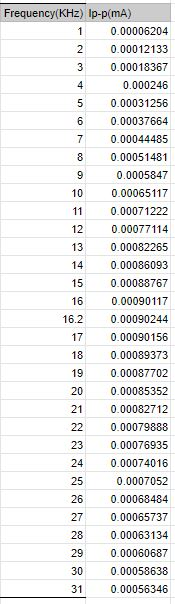
\includegraphics[width= 5cm]{Data_AC.JPG}
    \caption{Data collected from the experiment.}
    \label{fig:galaxy}
\end{figure}

The circuit has been analyzed by phasor form. The current analyze of the RLC circuit can be represented by following equation. 
% Circuit Analysis
\begin{equation}
\begin{aligned}
    I_{0} &= \frac{V_{0}}{\sqrt{R^2+(\omega L + \frac{1}{\omega C})^2}}\\
\end{aligned}
\end{equation}

Since values of R, L, C, \(I_0\), and \(V_0\) are known, RLC circuit which has been used in the experiment can be explained by using following equation.

\begin{equation}
\begin{aligned}
    I_{0} &= \frac{2}{\sqrt{(10 \text{ K} \Omega )^2+(\omega 10 \text{ mH} + \frac{1}{\omega 10 \text{ nF}})^2}}\\
\end{aligned}
\end{equation}

The total impedance of the series RLC circuit is
\begin{equation}
\begin{aligned}
    \omega &= 2 \pi f \\
    R + L + C &= R + j \omega L + \frac{1}{j \omega C}
\end{aligned}
\end{equation}

The circuit shows resonance behavior when the impedance of the Inductor and Capacitor is minimized, because the current goes directly through the Resistor.

\begin{equation}
\begin{aligned}
    \omega &= 2 \pi f \\
    R + L + C &= R + j \omega L + \frac{1}{j \omega C} \\
\end{aligned}
\end{equation}

When the impedance of L and C is minimized is

\begin{equation}
\begin{aligned}
    j \omega L + \frac{1}{j \omega C} &= 0 \\
    j( \omega L + \frac{1}{- \omega C}) &= 0 \\
    \omega L + \frac{1}{- \omega C} &= 0 \\
    \omega ^2 = \frac{1}{LC}
\end{aligned}
\end{equation}

Since the \( \omega = 2 \pi f \) ,

\begin{equation}
\begin{aligned}
    (2 \pi f) ^2 = \frac{1}{LC} \\
    4 \pi ^2 f^2 = \frac{1}{LC} \\
    f = \frac{1}{2 \pi \sqrt{LC} } \\
\end{aligned}
\end{equation}

Therefore, expected resonance frequency of the circuit is
\begin{equation}
    f = \frac{1}{2\pi \sqrt{LC}} =\frac{1}{2\pi \sqrt{10^(-2)*10^(-8)}} = 16   \text{ KHz}
\end{equation}

MATLAB code was used to plot simulation and experiment result. The following set of code is used to create a graph, and Figure 4 is the result of the MATLAB code.
\lstinputlisting[language=Matlab]{REUSimulCode.m}

%Figure 4
\begin{figure}[htp]
    \centering
    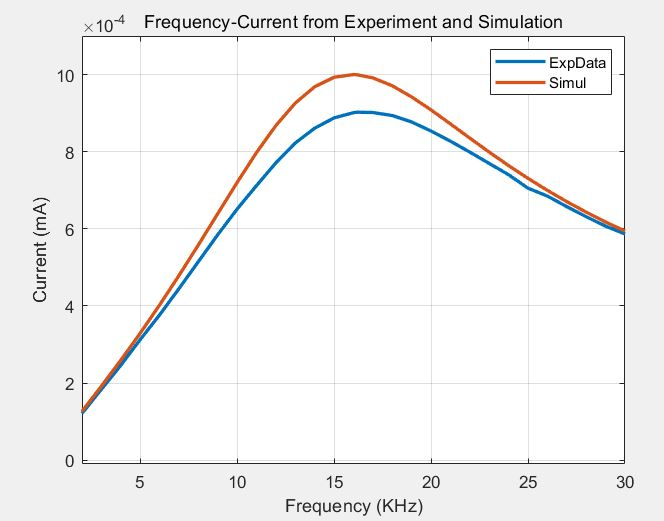
\includegraphics[width= 15cm]{lessErrorRLCsimul.JPG}
    \caption{Plot of the output current across the 1000 $k\Omega$ resistor, with Experimental data and Simulation data.}
    \label{fig:galaxy}
\end{figure}

The measured resonance frequency is 16.2 kHz, therefore, the resonance frequency matches the expectation.
The data from experiment shows the expected graph. The maximum voltage is measured at the frequency of 16.2 kHz and the value is 902.44 mV.


%Figure 5
\begin{figure}[htp]
    \centering
    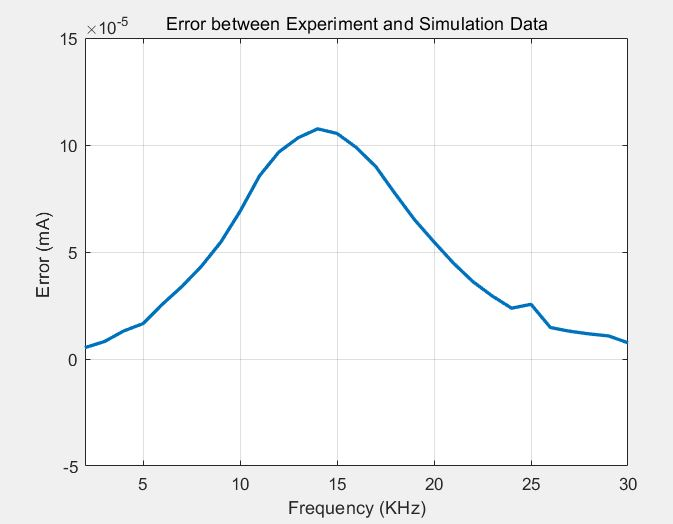
\includegraphics[width= 15cm]{ErrorPlot_Updated.JPG}
    \caption{Error between simulation and experiment data.}
    \label{fig:galaxy}
\end{figure}

As shown in the Figure 5, the error between experimental data and simulation data tends to be larger as it goes to resonance frequency. The source of the error is unknown, but is consistent with some nonlinearity in the current measurement.
\end{document}
